\documentclass{standalone}
\usepackage{tikz}

\begin{document}
\definecolor{pyplotC0}{RGB}{31,119,180}
\newcommand{\biquad}[1]{\protect\tikz[baseline=0ex]
  \protect\draw [draw=gray, very thick, scale=0.60, rounded corners=0.5mm]
  (0, 0) -- (#1, 0) -- (#1+0.25, 0.3) -- (1.25, 0.3) {};}
\newcommand{\shelf}{\protect\tikz[baseline=0ex]
  \protect\draw [ultra thick, scale=1, rounded corners=0.5mm, color=pyplotC0]
  (0, 0) -- (0.15, 0) -- (0.85, 0.6) -- (1, 0.6) {};}

\begin{plottikz}
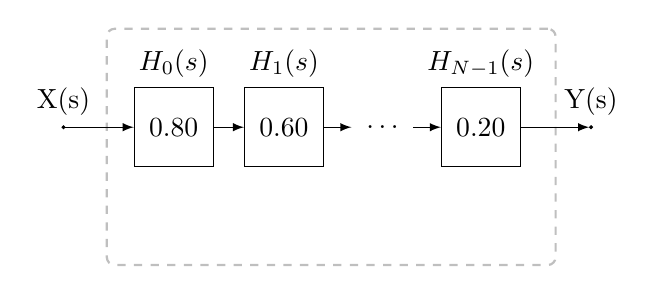
\begin{tikzpicture}
[scale=1, node distance=1.4cm, >=latex,
block/.style={
	rectangle, minimum size=10mm, minimum width=10mm, inner sep=2pt,
	draw=black},
largeblock/.style={
	rectangle, minimum size=8mm, minimum width=8mm, inner sep=3pt, thick,
	draw=gray!50, dashed, rounded corners=1mm},
dot/.style={
	circle, minimum size=1pt, inner sep=0pt,
	fill=black, draw=black}]

% coordinates
\coordinate (input) at (0, 0);
\coordinate [right of=input] (h0);
\coordinate [right of=h0] (h1);
\coordinate [right of=h1, node distance=2.5cm] (hN);
\coordinate [right of=h1, node distance=1.25cm] (dots);
\coordinate [right of=hN] (output);
\coordinate [right of=h0, node distance=2cm, yshift=-0.25cm] (cascade);

% input and output nodes
\node [dot, label={X(s)}] (In) at (input) {};
\node [dot, label={Y(s)}] (Out) at (output) {};

% cascade
\node [largeblock, minimum size=3cm, minimum width=5.7cm,
       label={[yshift=-2.85cm] \shelf}]
       (Cascade) at (cascade) {};

% biquads
\node [block, label={[yshift=0] $H_{0}(s)$}] (H0) at (h0) {\biquad{0.80}};
\node [block, label={[yshift=0] $H_{1}(s)$}] (H1) at (h1) {\biquad{0.60}};
\node [block, label={[yshift=0] $H_{N-1}(s)$}] (HN) at (hN) {\biquad{0.20}};


% signal flow
\draw [->] (In) -- (H0);
\draw [->] (H0) -- (H1) node [above, pos=0.5] {};
\draw [->] (H1.east) -- ++(0.35, 0) {};
\draw [<-] (HN.west) -- ++(-0.35, 0) {};
\draw [->] (HN) -- (Out) node [above, pos=0.5] {};
\node at (dots) {$\ldots$};

\end{tikzpicture}
\end{plottikz}

\end{document}
